Comme le montre le listing de code \ref{annexe:p-edf}, je me suis appuyé sur la librairie \texttt{litmus/edf\_common.h} fournie dans \litmus. J'ai donc ensuite décidé d'implémenter un algorithme d'ordonnancement qui ne l'utilisait pas. J'ai donc choisi d'implémenter un algorithme RM (Rate Monotonic) partitionné. Cet algorithme est plus simple que P-EDF car il ne prend pas en compte les échéances destâches. Il suffit alors de trier lestâches par période croissante et de les ordonnancer en fonction de leur période. Cependant, cet algorithme ne permet pas de garantir l'ordonnançabilité destâches. En effet, il existe des ensembles detâches qui ne sont pas ordonnançables par cet algorithme alors qu'ils le sont par P-EDF. Cependant, cet algorithme est plus simple à implémenter et permet de se familiariser avec les fonctions de \litmus.


\subsubsection{Implémentation}

Pour implémenter un algorithme RM partitionné, j'ai du réimplémenté les fonctions de \\ \texttt{litmus/edf\_common.h} pour suivre l'ordonnancement RM. Notre algorithme P-EDF faisait appel aux fonctions :
\begin{itemize}
    \item \texttt{edf\_domain\_init}, qui initialise le domaine temps réel avec l'ordre qui régit la priorité des tâches
    \item \texttt{edf\_preemption\_needed}, qui vérifie si la tâche en cours d'exécutions doit être préemptée
\end{itemize}
J'ai donc implémenté les fonctions :
\begin{itemize}
    \item \texttt{rm\_domain\_init}
    \item \texttt{rm\_preemption\_needed}
\end{itemize}

\begin{lstlisting}[style=cstyle, caption={Fonction \texttt{rm\_domain\_init}}, label={annexe:rm_domain_init}]
void rm_domain_init(rt_domain_t* rt, check_resched_needed_t resched,
					release_jobs_t release)
{
	rt_domain_init(rt, rm_ready_order, resched, release);
}
\end{lstlisting}

La complexité de cette fonction se cache derrière la nouvelle fonction d'ordre implémenté sous le nom de \texttt{rm\_ready\_order}. Cette fonction est passé en paramètre à \texttt{rt\_domain\_init} et permet d'initialiser le domaine temps réel avec l'ordre qui régit la priorité des tâches sous RM. Comme le montre le listing de code \ref{annexe:rm_common}, cette fonction est simple et permet de trier les tâches par période croissante. En cas, d'égalité, la priorité est départagée par PID croissant (la tâche avec le PID le plus petit est la plus prioritaire). On effectue aussi d'autres vérifications sur les tâches comme leur nature (tâche temps réel ou non), si deux fois la même tâche est passée en argument, ou encore si une des tâche est \texttt{NULL} (cas ou qu'une seul tâche n'est présente).

\subsubsection{Résultats et essais}

En raison de la grande quantité de nouveau code, faire fonctionner cet algorithme à nécessité une plus grande phase de débogage. J'ai donc utilisé l'outil \textit{feather-trace} pour tracer l'ordonnancement réel de cet algorithme. De cela, j'ai pu déterminer les étapes qui ne fonctionnaient pas. Par exemple, voici un exemple d'un essai avec plusieurs problèmes : 
\begin{figure}[H]
    \centering
    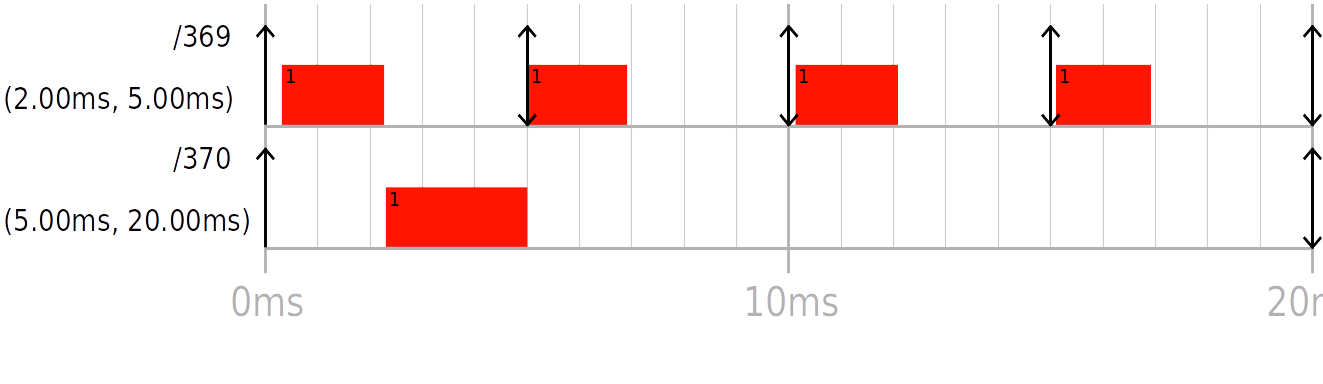
\includegraphics[width=0.9\textwidth]{Images/schedule_host=rock960_scheduler=DEMO_trace=notstoped.png}
    \caption{Exemple d'ordonnancement avec défauts}
\end{figure}

Premièrement, l’ordonnanceur ne stipule pas a \textit{feather-trace} la fin d'exécution d'une tâches. Cela peut être corrigé en  appelant \texttt{sched\_trace\_task\_completion(prev, budget\_exhausted);} lors de la fin d'un job.
Secondement, on peut voir que la deuxième tâche se fait préempter en $t=5ms$ par la première tâche, plus prioritaire. Cependant, l'exécution de cette deuxième tâche ne continue pas lorsque le processeur est libre. Cet erreur était alors du à une erreur de logique dans la fonctions principale d’ordonnancement dans laquelle je ne replaçait pas les tâches préemptés dans la \texttt{ready\_queue}.

Après ces erreurs corrigées voici le résultat de l’ordonnancement de 2 tâches par RM toutes deux lancées sur le même processeur :

\begin{figure}[H]
    \centering
    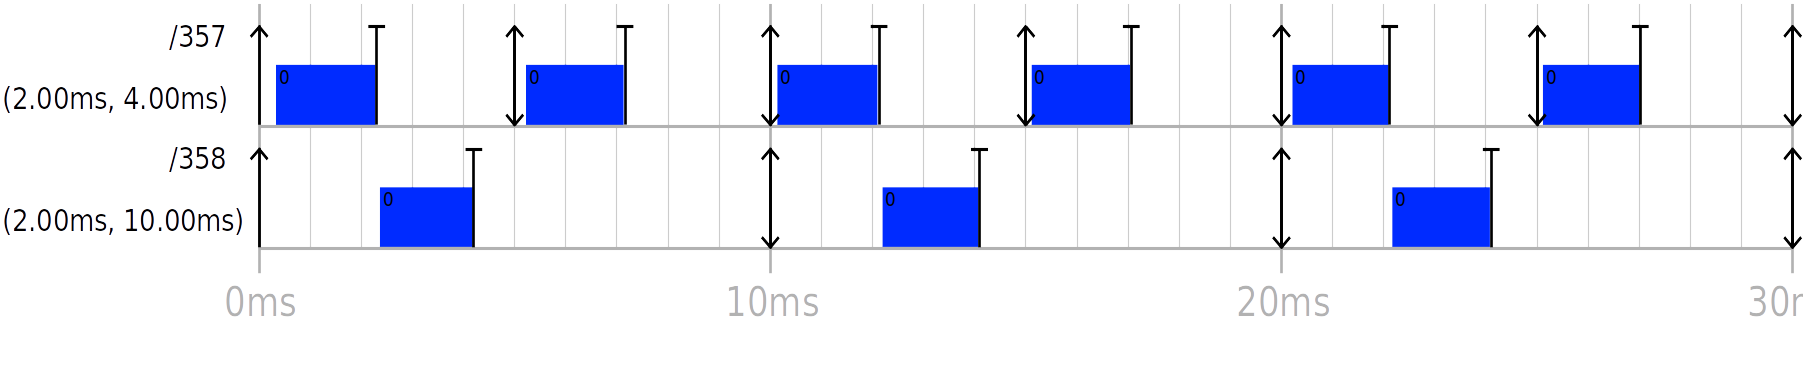
\includegraphics[width=0.9\textwidth]{Images/RM-No-Offset.png}
    \caption{Exemple d'ordonnancement de deux tâches par RM}
    \label{fig:rm-schedualibility-demo}
\end{figure}


On peut aussi lancer les tâches avec un \textit{offset} afin de voir si l'ordonnancement est correct. Ce décalage est donné en tant que paramètre a la commande \texttt{rt-spin} de \textit{liblitmus} (paramètre \texttt{-o}). Voici un exemple d'ordonnancement avec un \textit{offset} de 1ms pour la première tâche. Les tâches ont les mêmes pires temps d'exécution et les mêmes périodes que les tâches de la figure \ref{fig:rm-schedualibility-demo}.
\begin{figure}[H]
    \centering
    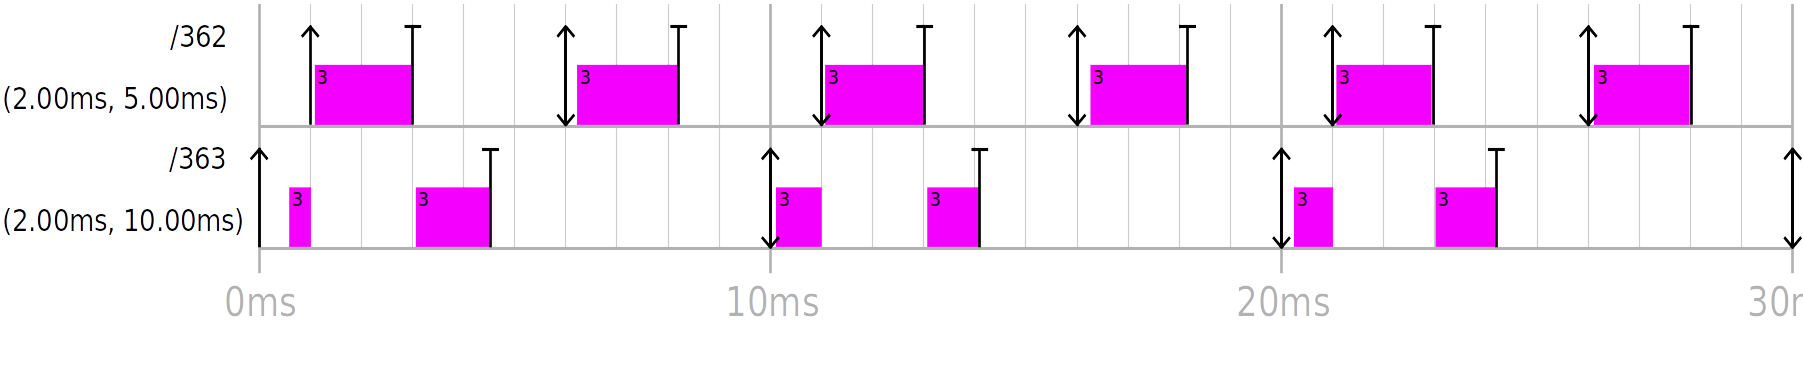
\includegraphics[width=0.9\textwidth]{Images/RM_OFFSET_SCHED.png}
    \caption{Exemple d'ordonnancement via RM avec un offset sur une tâche}
\end{figure}

On peut aussi lancer un plus grand nombre de tâches sur une multitude de processeurs (la carte de développement en ayant 6), et on obtient le tracé de tâches suivantes : 

\begin{figure}[H]
    \centering
    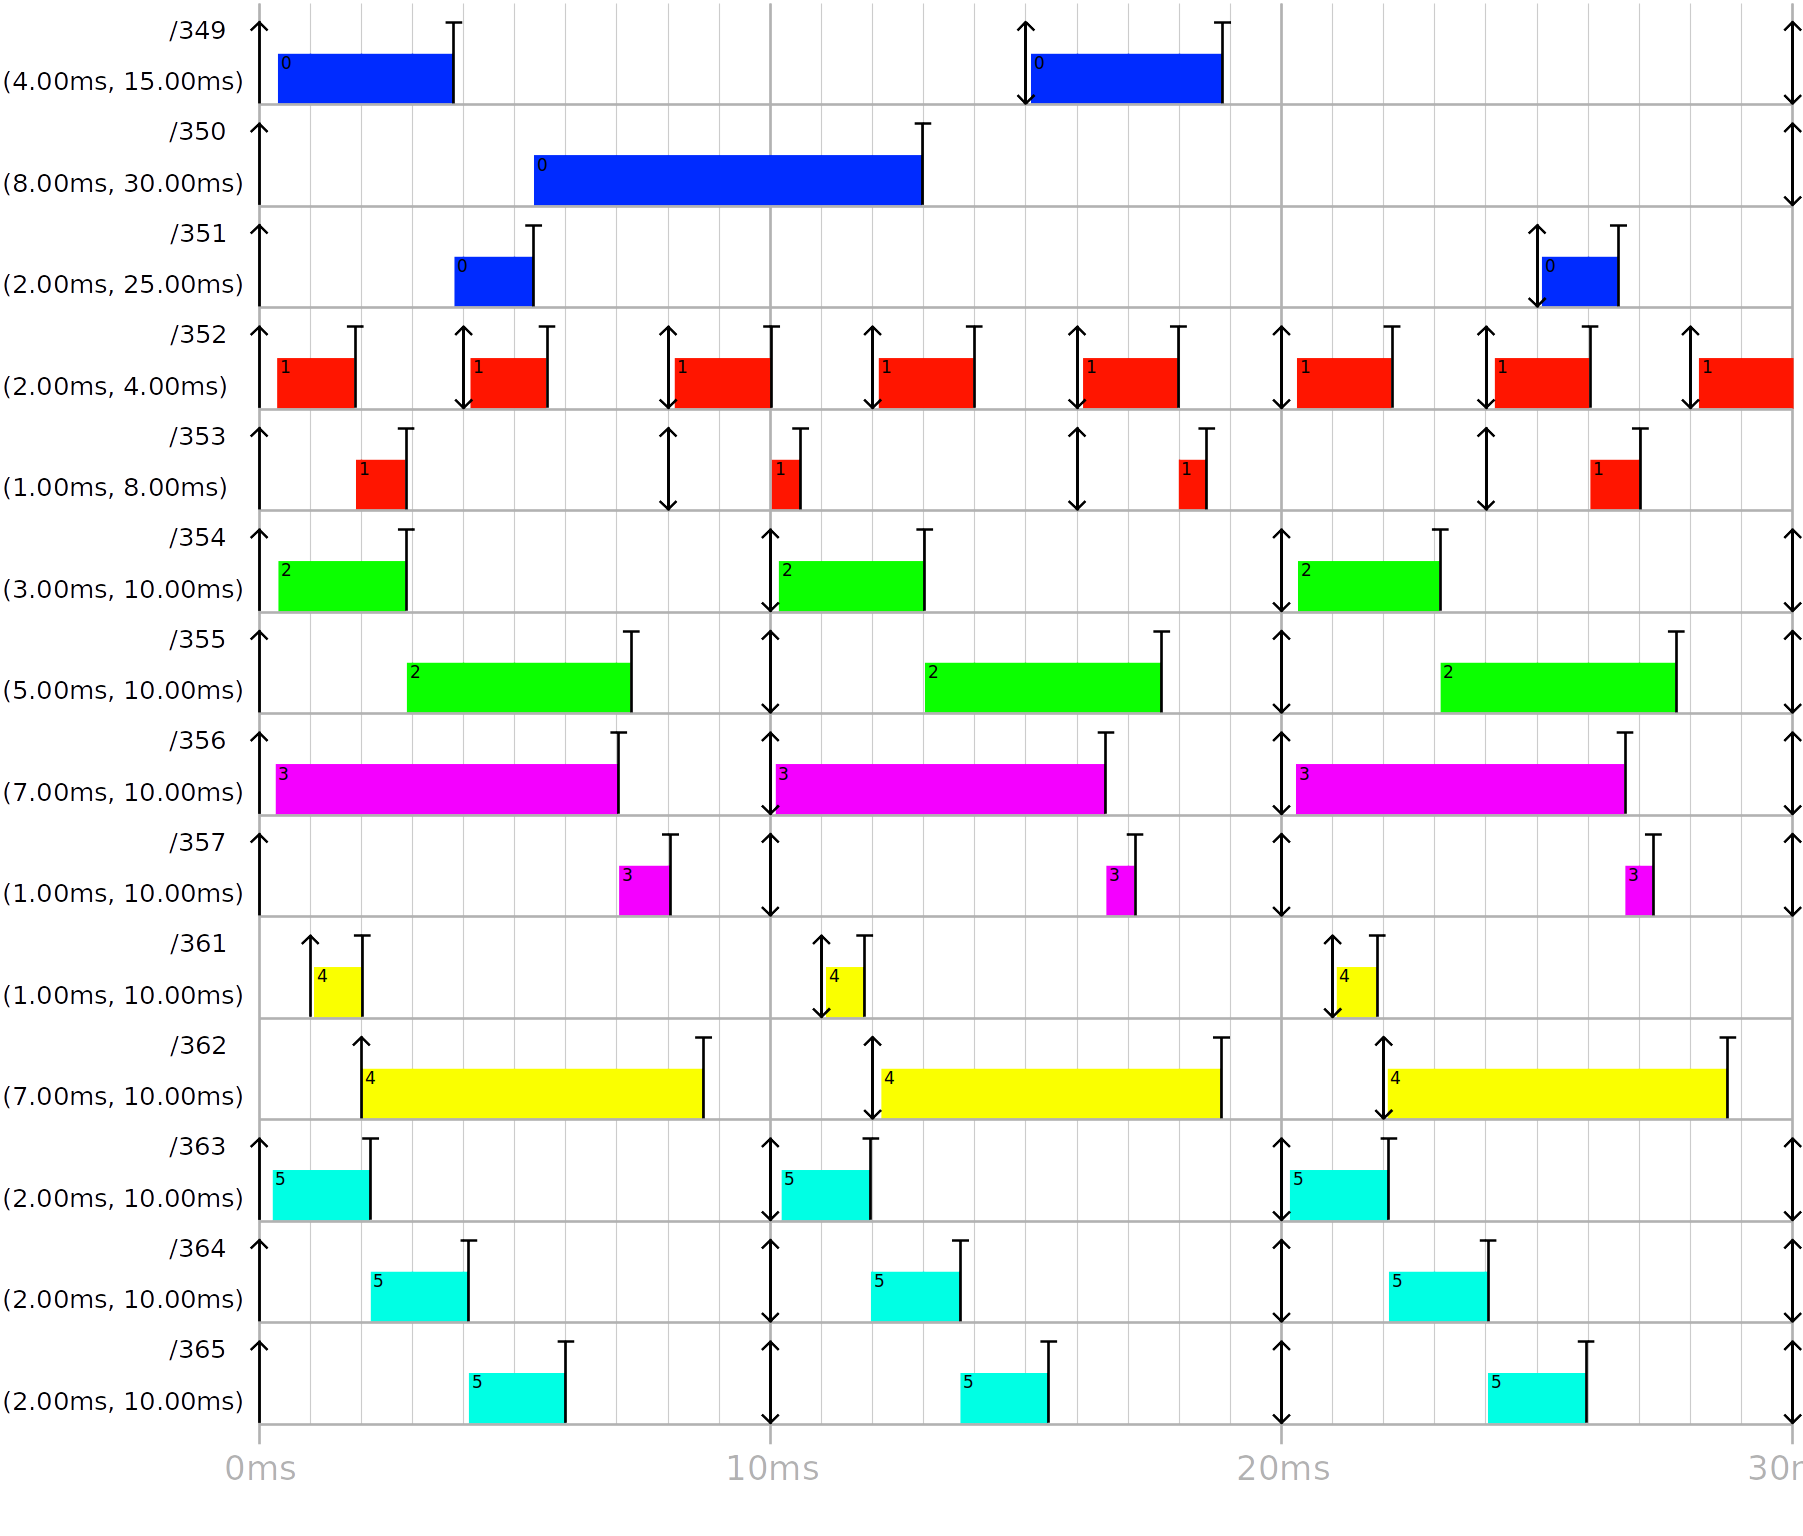
\includegraphics[width=0.9\textwidth]{Images/RM-bcp.png}
    \caption{Exemple d'ordonnancement d'un grand ensemble de tâches via RM}
\end{figure}


Enfin, on peut aussi voir ce qu'il se passe lorsque l'on cherche a ordonnancer les même tâches que celles que l'on à ordonnancé avec P-EDF et que l'on peut voir dans la figure \ref{fig:edf-schedualibility-demo}. Ces tâches sont non-ordonancables par RM et on obtient le tracé suivant :

\begin{figure}[H]
    \centering
    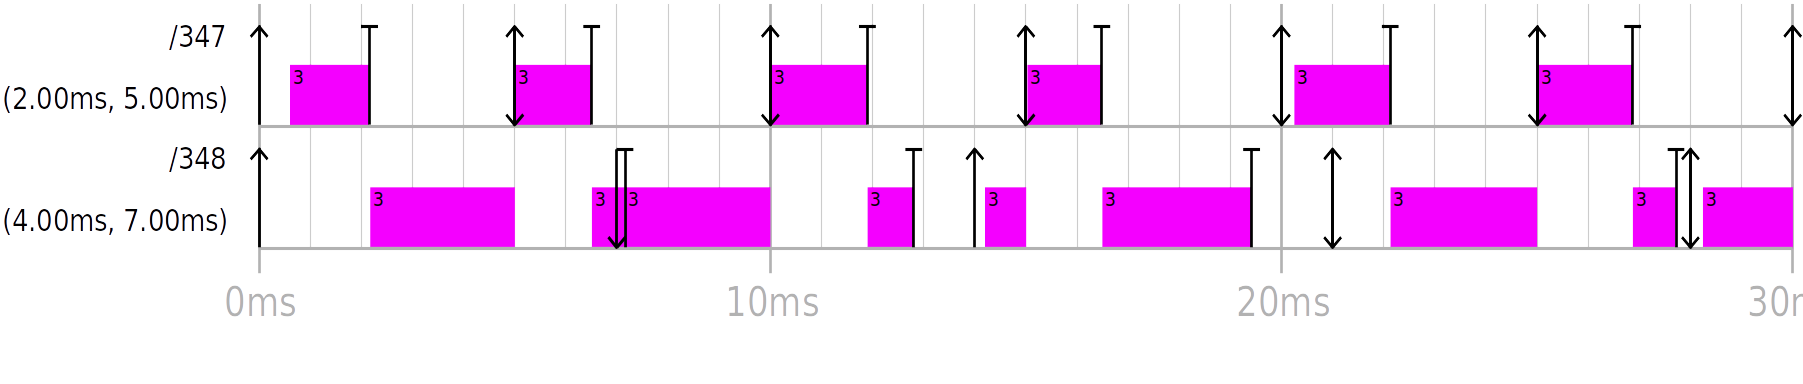
\includegraphics[width=0.9\textwidth]{Images/RM_rMerde.png}
    \caption{Exemple d'ordonnancement de tâches non-ordonnançables par RM}
\end{figure}

Les dépassement des échéances montrent bien que RM est moins performant que P-EDF car il ne permet pas d'ordonnancer toutes les tâches ordonnançables par P-EDF. Cependant, il est plus simple à implémenter et m'a permis de me familiariser avec les fonctions de \litmus. Mais, des résultats comme le pire temps de réponse d'une tâche est plus simple a obtenir analytiquement avec RM qu'avec P-EDF. Cela est du au fait que RM est plus simple à analyser que P-EDF et c'est pourquoi il est actuellement plus utilisé dans des domaines comme l'avionique.
